\documentclass[10pt,a4paper]{article}
\usepackage[utf8]{inputenc}
%\usepackage[french]{babel}
\usepackage[T1]{fontenc}
\usepackage{amsmath}
\usepackage{amsfonts}
\usepackage{amssymb}
\usepackage{verbatim}
\usepackage{graphicx}

\author{Donatien Dallery}
\title{La télédétection et GéoBretagne : méthodes, produits et analyses}
\begin{document}
\maketitle

\begin{abstract}
GéoBretagne a intégré des données de télédétection à son catalogue. Dans un premier temps, 4 produits sont disponibles : 
\begin{itemize}
\item un indice de végétation (NDVI) pour la distinction des surfaces végétales/non végétales
\item l'Evaporative Fraction (EF) pour estimer l'évaporation d'un sol et donc, son potentiel hydrique
\item la température moyenne sur 8 jours de jour et de nuit
\end{itemize}

Chacun de ces produits possède une dimension temporelle afin de suivre l'évolution de ces indices de manière intra et inter-annuelle. Le capteur MODIS a été choisi pour effectuer cette introduction à la télédétection.
\end{abstract}

\section{Introduction}

La définition officielle de la télédétection est « l’ensemble des connaissances et techniques utilisées pour déterminer des caractéristiques physiques et biologiques d’objets par des mesures effectuées à distance, sans contact matériel avec ceux-ci » (COMITAAS, 1988).\smallbreak

La notion de "sans contact matériel avec ceux-ci" correspond à l'acquisition d'informations sur la Terre à partir de satellites, avions, drones ou simplement d'un appareil photo jeté en l'air (à vos risques et périls). Pour l'étude d'autres planètes, les télescopes effectuent également de la télédétection étant donné qu'ils ne sont pas en contact avec celles-ci.\smallbreak

L'acquisition d'informations s'opère par la mesure du spectre électromagnétiques dans les domaines (figure \ref{spectreElectro}) :

\begin{itemize}
\item du visible pour l'oeil humain, comme un appareil photo
\item de l'invisible pour l'oeil humain :
\begin{itemize}
\item l'infrarouge (télécommande, capteur thermique)
\item les micro-ondes (téléphone, radar)
\end{itemize}
\end{itemize}

\begin{figure}[!h]
\centering
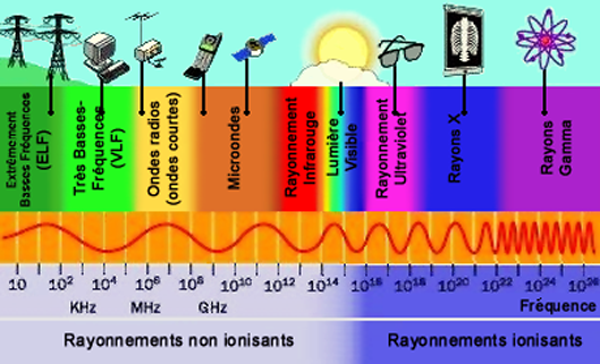
\includegraphics[scale=0.6]{img/spectre-electromagnetique.png}
\caption{Représentation du spectre électromagnétique (source : astronoo.com)}
\label{spectreElectro}
\end{figure}

Dans le cadre de cette introduction à la télédétection, les données employées se situent dans les domaines du visible et de l'invisible (infrarouge).

\subsection{Capteur MODIS}

Le capteur MODIS est un spectroradiomètre imageur (un appareil photo) se trouvant sur deux satellites (Terra et Aqua) (figure \ref{modis}) mis en service par la NASA dont les données sont diffusées gratuitement par l'United States Geological Survey (USGS) .

\begin{figure}[!h]
\centering
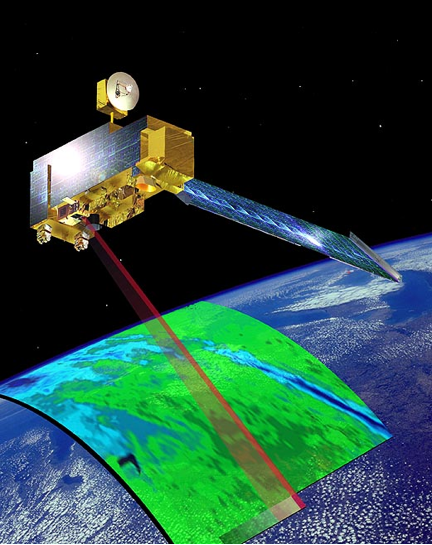
\includegraphics[scale=0.4]{img/modis.png}
\caption{Représentation du satellite Terra avec le capteur MODIS}
\label{modis}
\end{figure}

Ce capteur dispose d'une résolution spatiale allant de 250 mètres à 1 kilomètre avec une résolution temporelle journalière. Une image (tuile) de ce capteur couvre 2330 km$^2$ (figure \ref{modisGrid}).

\begin{figure}[!h]
\centering
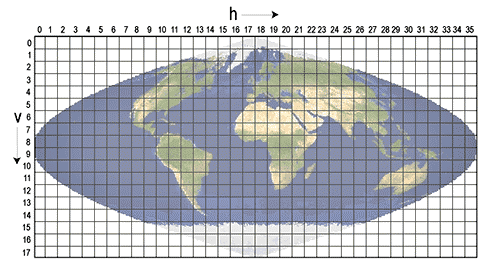
\includegraphics[scale=0.7]{img/modisGrid.png}
\caption{Grille d'acquisition des images MODIS}
\label{modisGrid}
\end{figure}

Ce capteur a été sélectionné pour plusieurs de ses caractéristiques, bien que généralement, les études utilisant des images MODIS sont effectuées sur des paysages ouverts et non fragmentés en petites parcelles (Morton et al., 2006; Wardlow et al., 2006) comme la Bretagne :
\begin{itemize}
\item une résolution temporelle journalière et des synthèses de 8 jours (valeur moyenne ou maximale, selon les produits, sur 8 jours)
\item un capteur acquérant des informations dans l'infrarouge thermique (nécessaire pour calculer EF)
\item des archives importantes (il est possible d'avoir des données à partir de l'an 2000) pour l'aspect temporel mis en avant sur GéoBretagne
\end{itemize}

\subsection{Produits disponibles sur GéoBretagne}

Les premiers produits diffusés ont tous une dimension temporelle avec un pas de temps de 8 jours.

\subsubsection{NDVI}

Le NDVI (Rouse and Haas, 1973; Tucker, 1979) est un indice de végétation standard dans l'étude de la végétation (Gao, 1996). Cet indice se calcule avec les bandes électromagnétiques du rouge (R) et du proche infrarouge (Pir). Le résultat est normalisé entre -1 (autre que végétation tel l'eau) et 1 (végétation dynamique).\smallbreak

\begin{center}
\textrm{NDVI}=$ \frac{Pir-R}{Pir+R} $
\end{center}\smallbreak

Ces bandes sont employées d'après l’interaction des bandes du rouge et du proche infrarouge avec la végétation. L'énergie de la bande du rouge est absorbée par la végétation (chlorophylle), au contraire du proche infrarouge qui est réfléchi par l'eau contenu dans la végétation (parenchyme lacuneux). De même, plus la végétation sera dynamique, plus il y aura d'absorption dans la bande du rouge et de réflectance pour celle du proche infrarouge.\smallbreak

La figure \ref{signSpectr} permet de distinguer la réflectance type de la végétation (en vert), de l'eau (en bleu) et du sol (en rouge). Les bandes sont représentées par les zones grisées avec celle du rouge (3) et du proche infrarouge (4). Ainsi, le NDVI calcule la différence de réflectance entre les 2 bandes. Plus cette différence est importante (comme sur la figure \ref{signSpectr}), plus la végétation sera dynamique et le NDVI proche de 1. Concernant l'eau, sa réflectance est nulle dans le proche infrarouge, ayant pour effet d'avoir un NDVI inférieur à 0. Pour le sol, selon différents paramètres (couleur, composition, humidité, rugosité) les réflectances dans le rouge et le proche infrarouge sont équivalentes, induisant un NDVI proche de 0.\smallbreak

\begin{figure}[!h]
\centering
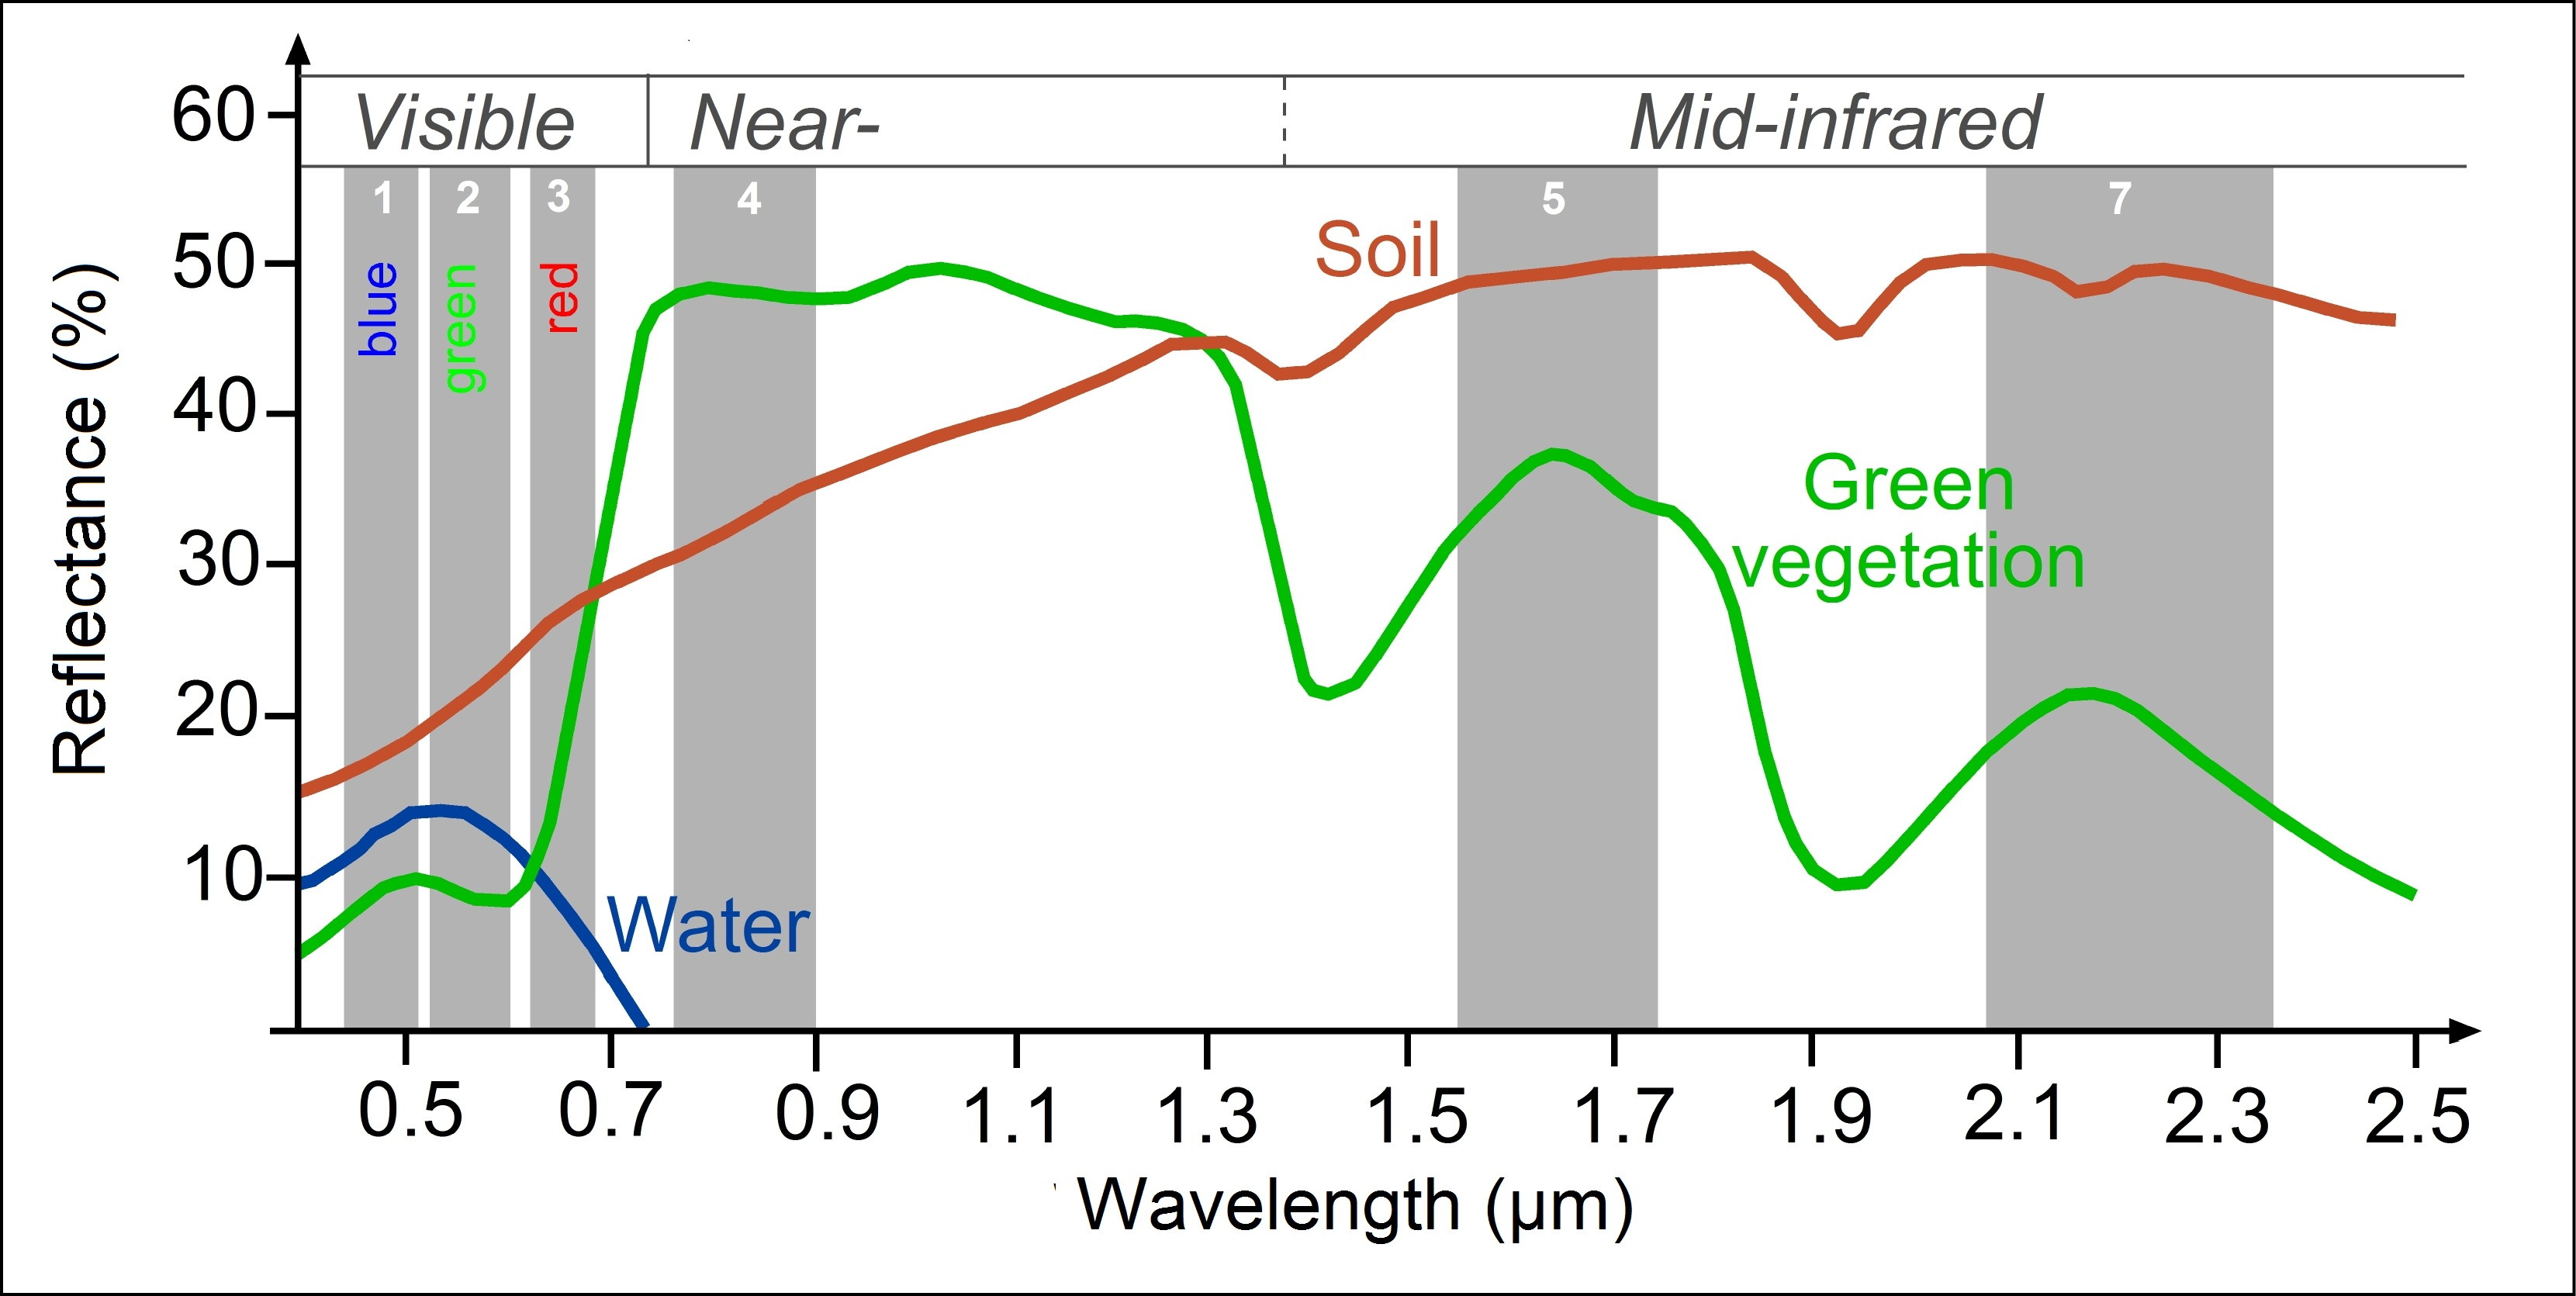
\includegraphics[scale=0.4]{img/spectral_signatures.jpg}
\caption{Signatures spectrales du sol, de l'eau et de la végétation vis à vis du spectre électromagnétique entre 350 et 2500nm. Source: SEOS Project}
\label{signSpectr}
\end{figure}

Cet indice permet d'effectuer une classification de l'occupation du sol. De part l'aspect temporel mis en avant sur GéoBretagne, cet indice permet également de suivre la phénologie de la végétation. De cette manière, il est possible de déterminer l'usage des sols (Patakamuri et al., 2014).

\subsubsection{Evaporative Fraction}

L'Evaporative Fraction est un indice permettant d'estimer la capacité d'un sol à évaporer et donc son humidité (Bastiaanssen et al., 2003; Nutini et al., 2014). Cet indice se calcule avec le NDVI et des mesures de températures de jour et de nuit que ce soit par télédétection (infrarouge thermique) ou non (thermomètre). Les valeurs de cet indice vont de 0 (surface non évaporante) à 1.26 (surface très évaporante). Le modèle S-SEBI (Roerink et al., 2000) et le coefficient de Priestley-Taylor sont employés pour calculer EF.\smallbreak

De cette manière, il est possible de définir le stress hydrique de la végétation, particulièrement à partir d'une série temporelle (disponible sur GéoBretagne). En effet, si le sol évapore beaucoup, alors que les précipitations sont faibles, il est probable d'observer une sécheresse. Cet indice est également employé pour estimer l'évapotranspiration et la biomasse à partir de modèles (Nutini et al., 2014).

\subsubsection{Température de jour et de nuit}

Ces deux données sont mis à disposition par l'USGS-LP DAAC sous la dénomination du produit MODIS MOD11A2. Ces données correspondent à la température moyenne (en kelvin) par temps clair sur 8 jours de jour et de nuit. Cette donnée est utilisée pour calculer EF. Ces températures sont également disponibles sur GéoBretagne étant donné que plusieurs informations sont accessibles, tel les îlots de chaleur urbains avec les températures de nuit ou les milieux humides/aquatiques avec les températures de jour ou de nuit étant donné leur amplitude thermique plus faible que le sol et la végétation.

\section{Méthodologie}

La chaîne de traitement développée pour générer et rendre accessible ces produits sur GéoBretagne se divise en 3 parties :

\begin{enumerate}
\item Téléchargement des images MODIS
\item Génération des produits
\item Publication sur un GeoServer
\end{enumerate}

Remarque : Pour tous les produits à publier sur le Geoserver, il est impératif de respecter cette nomenclature : Nom\_YYYYMMDD.tif. Dans le cas contraire, le GeoServer (dans la configuration actuelle), ne sera pas capable de gérer l'aspect temporel de l'image.

\subsection{Téléchargement des données MODIS}

Les produits MODIS nécessaires pour les traitements sont MOD09Q1 (bandes du rouge et du proche infrarouge) à 250m de résolution spatiale et MOD11A2 (température de jour et de nuit) à 1km. La tuile à télécharger est la h17v04. Ces produits sont disponibles sur la plateforme de téléchargement LP DAAC de l'USGS \verb!https://lpdaac.usgs.gov/data_access/data_pool.! Les archives pour ces produits débutent au 18 Février 2000 et une nouvelle image est ajoutée tous les 8 jours (approximativement).\smallbreak

Le téléchargement des images repose sur différents critères, c'est à dire le site de téléchargement (fixe), le produit (fixe), la tuile (fixe) et la date du produit (variable) dont voici le fonctionnement (figure \ref{orgDL}) :\newpage

\begin{figure}[!h]
\centering
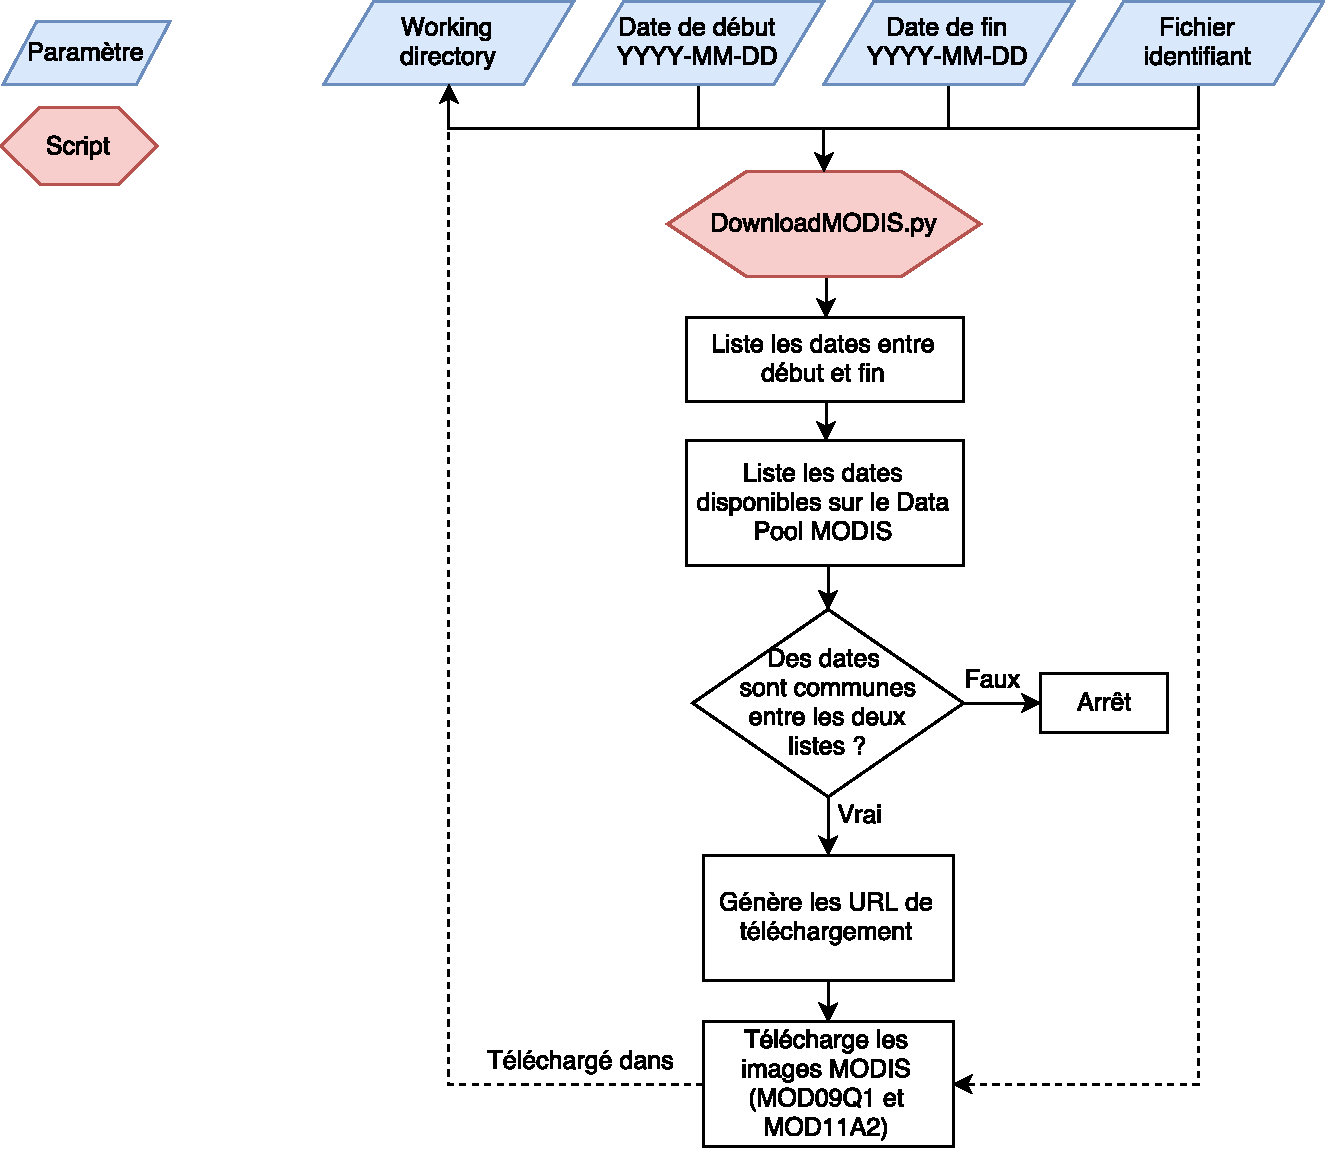
\includegraphics[scale=0.5]{img/orgDownload.pdf}
\caption{Organigramme des étapes nécessaires pour le téléchargement des produits MODIS.}
\label{orgDL}
\end{figure}

\subsection{Génération des produits}

La production des produits diffusés s'opère en 3 étapes :

\begin{enumerate}
\item Contrôle des dates déjà traitées
\item Prétraitement des images
\item Génération des produits
\end{enumerate}

Le fonctionnement du script pour réaliser les produits diffusés sur GéoBretagne est le suivant (figure \ref{orgIndex}) :\newpage

\begin{figure}[!h]
\centering
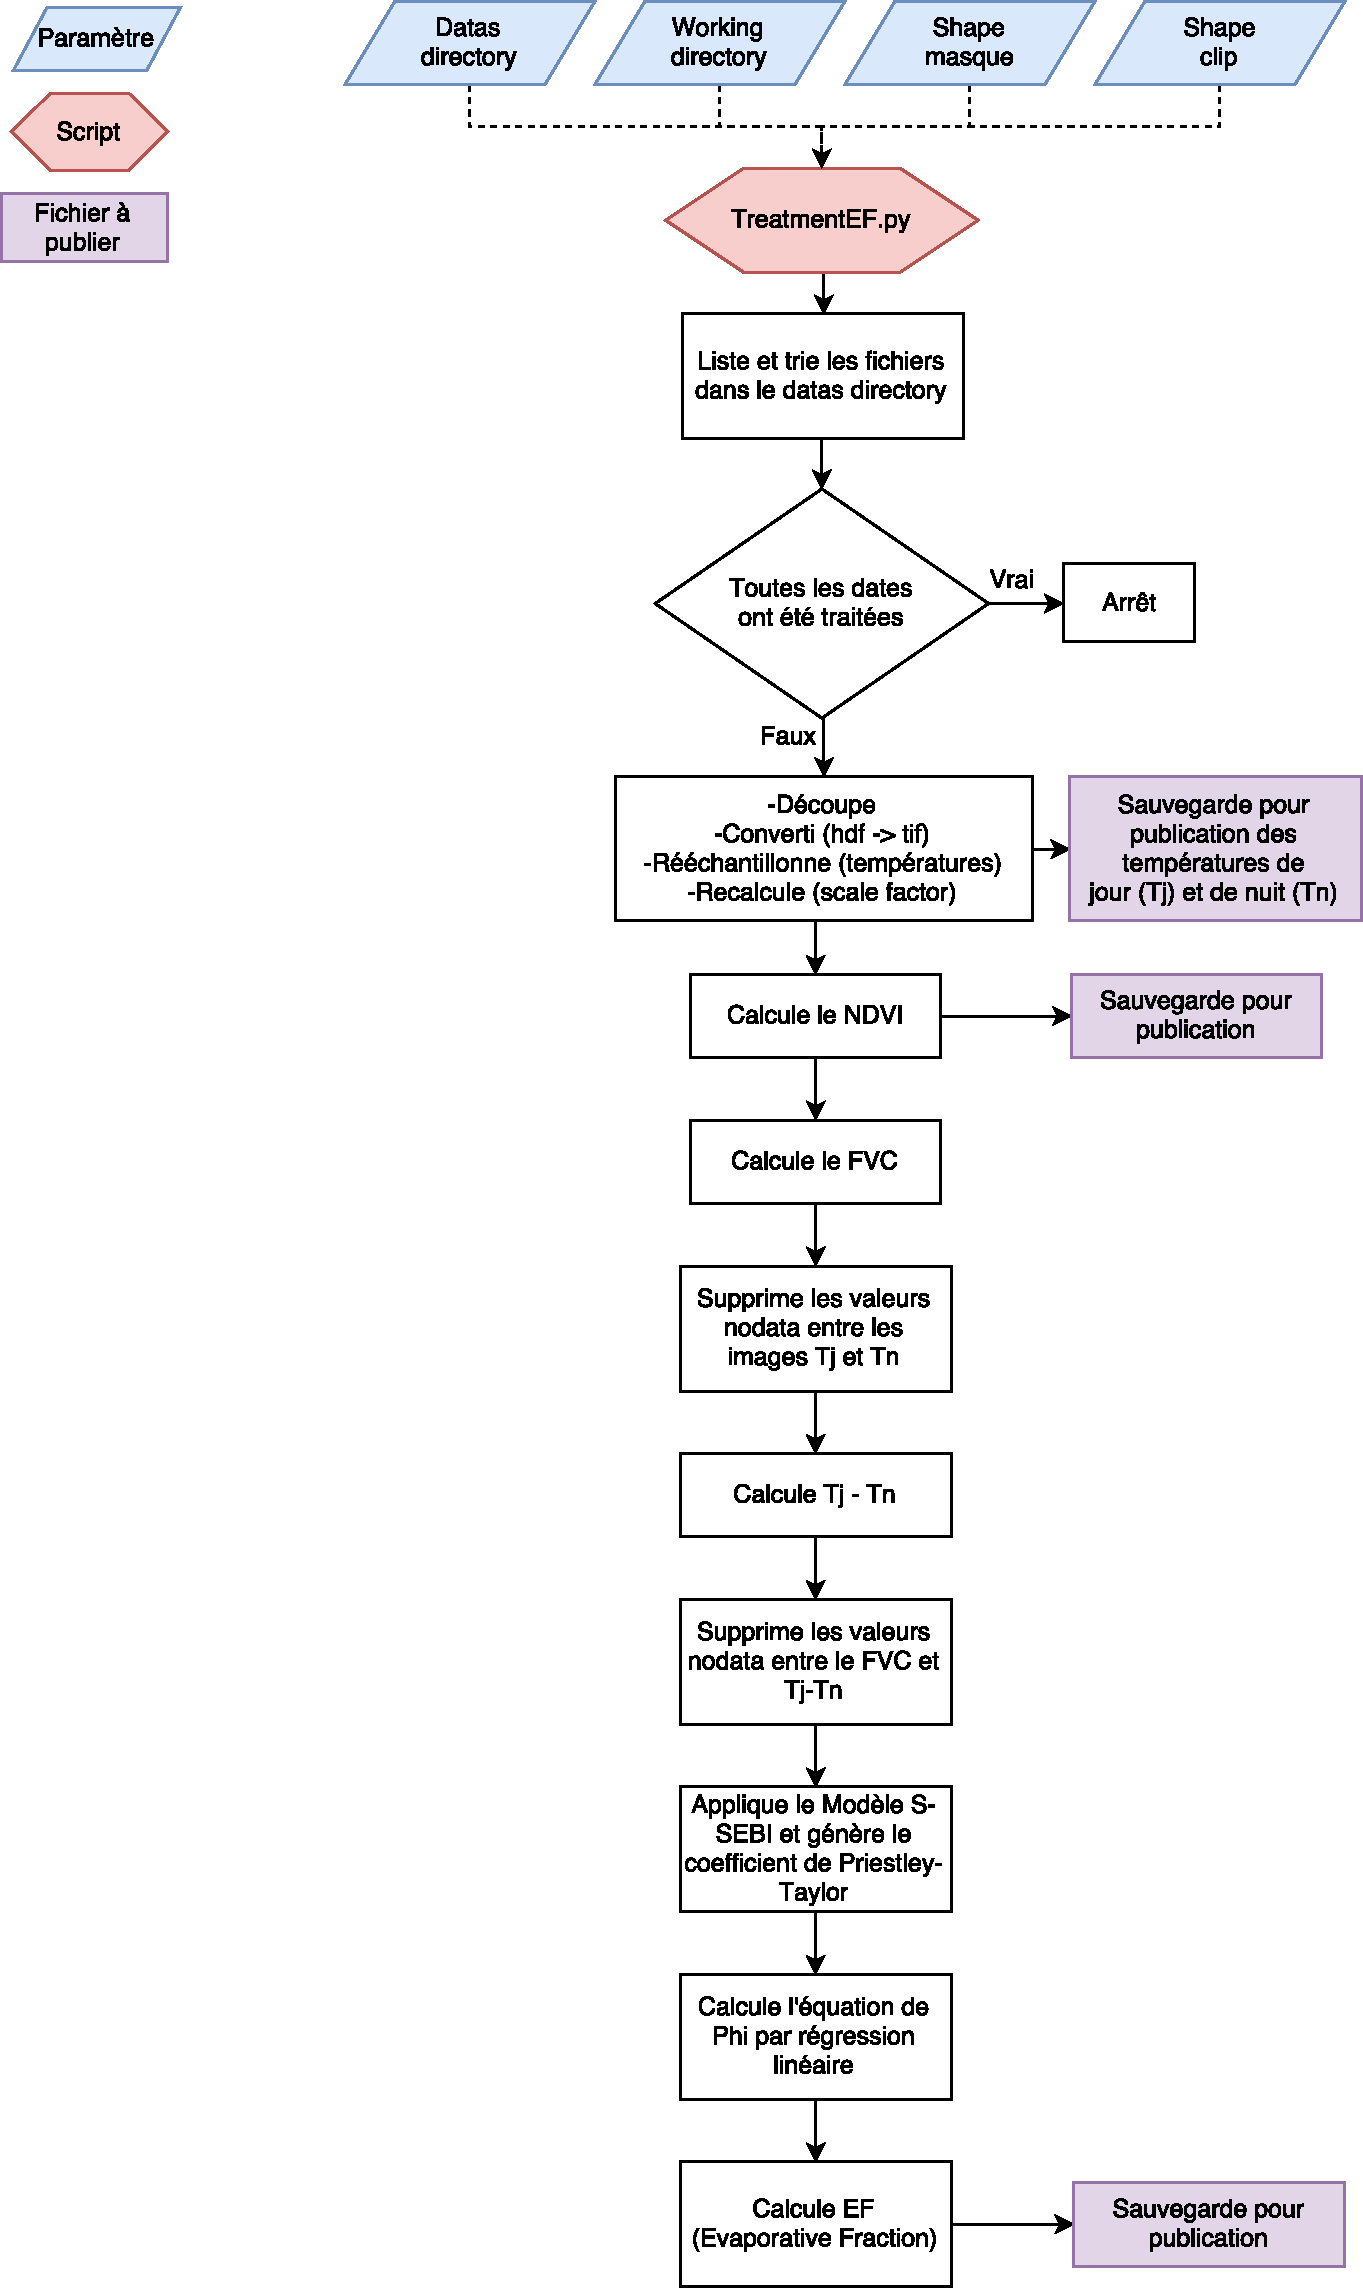
\includegraphics[scale=0.48]{img/orgIndices.pdf}
\caption{Organigramme des étapes pour la génération des indices diffusés sur GéoBretagne.}
\label{orgIndex}
\end{figure}

Les paramètres en entrée du script sont :

\begin{itemize}
\item le dossier contenant les images téléchargées précédemment
\item le dossier où enregistrer les produits générés
\item un shapefile pour découper les images
\item un shapefile pour masquer les pixels de la mer
\end{itemize}

\subsubsection{Prétraitements}

Les images téléchargées nécessitent des prétraitements avant de générer les produits. Ils consistent à :

\begin{itemize}
\item découper les images à l'échelle de la Bretagne et supprimer les pixels de la mer
\item changer le format de fichier des images (hdf vers tif)
\item rééchantillonner les images des températures (1km vers 250m)
\item recalculer les valeurs selon un facteur indiqué sur le site de l'USGS
\end{itemize}

Les températures sont directement publiables, aucun traitement supplémentaire ne sera effectué.

\subsubsection{NDVI}

L'étape suivante consiste à calculer le NDVI. Pour les étapes suivantes, les valeurs inférieures à 0 et supérieures à 1 (quelques pixels de mer non masqués ayant des valeurs aberrantes) sont supprimés. Le NDVI ne dispose alors que de valeurs allant de 0 à 1, caractéristique nécessaire pour calculer EF. Ce changement de valeurs n'est pas répercuté sur le produit NDVI diffusé sur GéoBretagne.

\subsubsection{Modèle S-SEBI et coefficient Priestley-Taylor}

Pour pouvoir appliquer le modèle S-SEBI et générer le coefficient de Priestley-Taylor, il est nécessaire de calculer le Fractional Vegetation Cover (FVC) et calculer la température de surface (figure \ref{graphFVCTemp}).

\begin{figure}[!h]
\centering
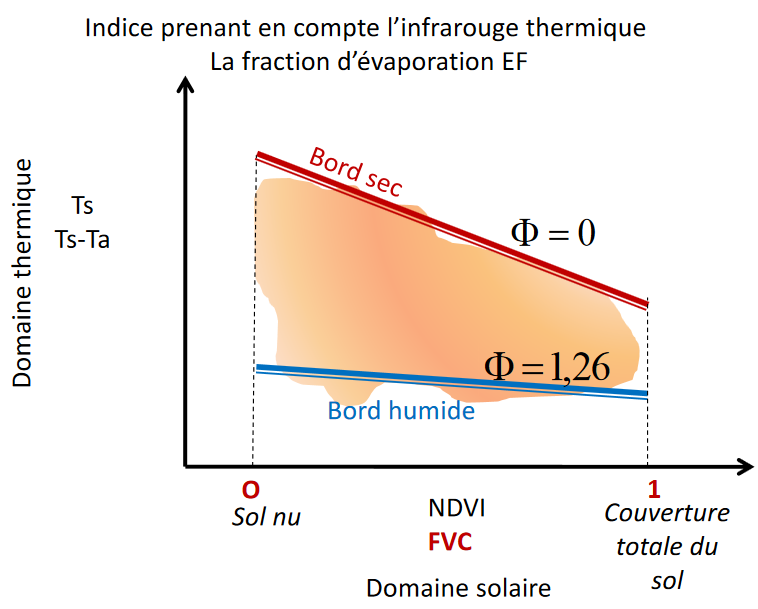
\includegraphics[scale=0.313]{img/graph_fvc_temp.png}
\caption{Graphique représentant le modèle S-SEBI pour générer le coefficient de Priestley-Taylor afin de calculer l'Evaporative Fraction.}
\label{graphFVCTemp}
\end{figure}

\begin{enumerate}
\item[(a)]FVC \medbreak
Cet indice représente la couverture de la végétation sur le sol. Plus l'indice est proche de 1, plus le sol est recouvert par la végétation et inversement. Il se calcule de la manière suivante :
\begin{center}
\textrm{FVC}=$ (\frac{NDVI-minNDVI}{maxNDVI-minNDVI})^2 $
\end{center}\smallbreak

\item[(b)]Température Tj - Tn \medbreak
Pour calculer cette valeur, il est d'abord nécessaire de reporter les pixels sans données d'une image sur l'autre. Si cette étape n'est pas effectuée, des températures aberrantes vont être générées suite à la soustraction. Ces pixels sans données seront également à supprimer sur le FVC avant d'opérer le traitement suivant.
\end{enumerate}

Avec le FVC et l'image Tj - Tn, nous pouvons produire le nuage de point des valeurs (figure \ref{graphFVCTemp}) et récupérer uniquement les points composant les bords sec et humides pour calculer le coefficient de Priestley-Taylor. Ce coefficient ainsi que l'équation de droite associé sont obtenus après une double interpolation pour ces deux bords suivis d'une régression linaire entre eux (figure \ref{graphPriestley}).

\begin{figure}[!h]
\centering
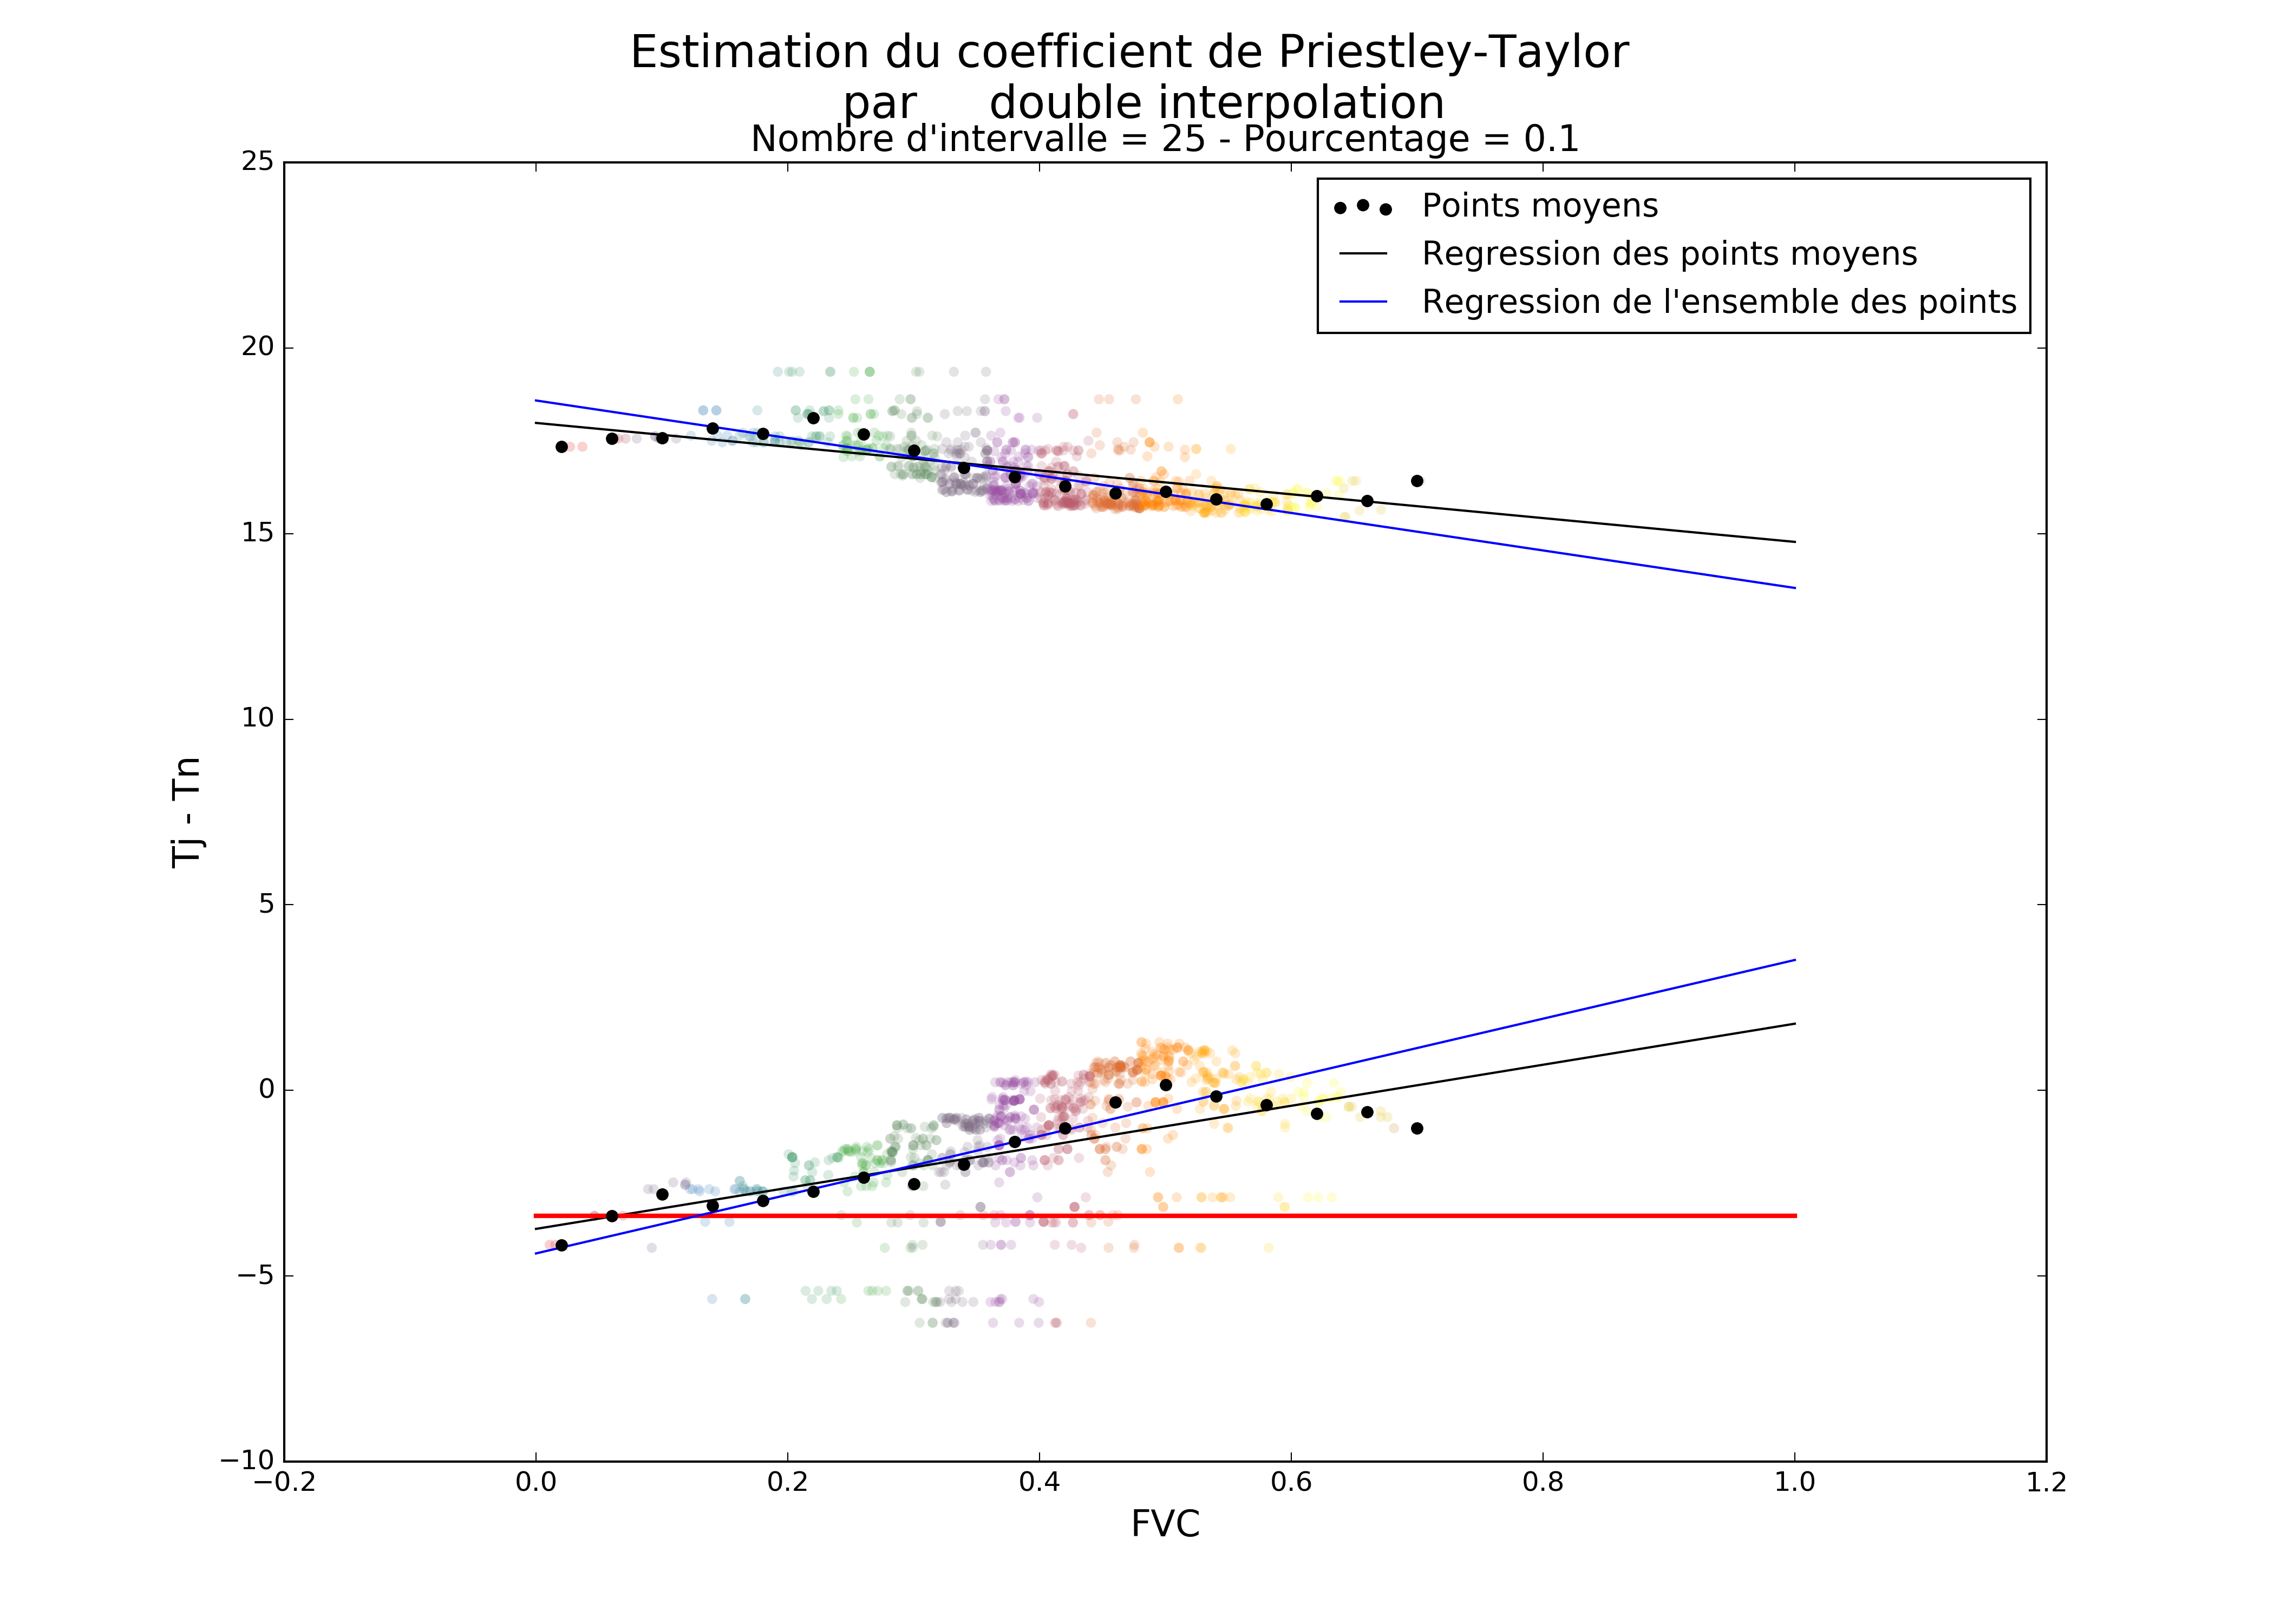
\includegraphics[scale=0.35]{img/graph_priestley.png}
\caption{Estimation du coefficient de Priestley-Taylor par double interpolation afin de calculer l'Evaporative Fraction.}
\label{graphPriestley}
\end{figure}

\subsubsection{Evaporative Fraction}

Le calcul de cet indice se déroule en plusieurs étapes :
\begin{enumerate}
\item Calcul de la température maximale d'après l'équation de droite obtenue précédemment
\item Avec cette température, calcul du coefficient de Priestley-Taylor :
\begin{center}
\textrm{Phi}=$ (\frac{Tmax-TjTn}{Tmax-Tmin})*1.26 $
\end{center}\smallbreak
\item Calcul de la température moyenne :
\begin{center}
\textrm{Tmoy}=$ ({Tj+Tn})/2 $
\end{center}\smallbreak
\item Calcul de ESatTa :
\begin{center}
\textrm{ESatTa}=$ (1000*exp(52.57633-(\frac{6790.4985}{Tmoy})-5.02808*log(Tmoy))) $
\end{center}\smallbreak
\item Calcul de delta :
\begin{center}
\textrm{delta}=$ (\frac{ESatTa}{Tmoy}) * ((\frac{6790.4985}{Tmoy})-5.02808) $
\end{center}\smallbreak
\item Calcul de EF :
\begin{center}
\textrm{EF}=$ (\frac{delta}{(delta+66)})*Phi $
\end{center}\smallbreak
\end{enumerate}

Nous obtenons alors une image renseignant sur la capacité d'un sol à évaporer. L'étape suivante consiste alors à publier ces données sur un GeoServer.

\subsection{Publication des produits sur un GeoServer}

\subsubsection{Initialisation du workspace, du store et du répertoire de données pour des données temporelles}

Ci-dessous la démarche à adopter pour générer un store temporel avec des données formalisés pour celui-ci.

\begin{enumerate}
\item création du workspace de manière standard en nommant celui-ci.
\item copier, si elles n'ont pas été générée sur le GeoServer, les images dans un dossier accessible par celui-ci. De plus, ajouter dans ce dossier deux fichiers de configurations pour exploiter la dimension temporelle des images :
\begin{itemize}
\item indexer.properties avec :
\begin{itemize}
\item TimeAttribute=time (nom de l'attribut temporel)
\item ElevationAttribute=elevation (dans le cas d'une dimension altitudinale)
\item \verb!Schema=*the_geom:Polygon,location:String,!\newline \verb!time:java.util.Date,elevation:Integer!
\item PropertyCollectors=TimestampFileNameExtractorSPI \newline [timeregex](time)
\end{itemize}
\item timeregex.properties avec :
\begin{itemize}
\item regex=[0-9]{8} (pour indiquer que la date est au format YYYYMMDD)
\end{itemize}
\end{itemize}
\item création du store avec l'extension ImageMosaic et en indiquant de répertoire contenant les images et les deux fichiers de configuration
\item création du layer en renseignant :  :
\begin{itemize}
\item onglet Data : dans la cellule sorting "time D" pour trier les dates (time correspondant au nom de l'attribut indiqué dans indexer.properties) par ordre décroissant (D)
\item onglet Dimensions : activer le time et choisir une présentation "List"
\end{itemize}
\item le store temporel est configuré, la mise à jour passera par un script
\end{enumerate}

\subsubsection{Mise à jour d'un store temporel existant}

Un script effectue cette étape et possède 5 paramètres en entrée :

\begin{itemize}
\item l'url du Geoserver
\item le workspace du produit
\item le store du produit
\item un fichier d'identifiant pour le GeoServer
\item le répertoire sur le serveur contenant le produit à publier
\end{itemize}

Ce script publie un seul produit à la fois, il est donc à exécuter autant de fois que nécessaire.\smallbreak
Remarque : si les produits ne sont pas accessible par le GeoServer, il est impératif de les déplacer sur le serveur de celui-ci. De plus, ce script effectue uniquement une mise à jour, le workspace et le store sont à générer manuellement. \newpage

\begin{figure}[!h]
\centering
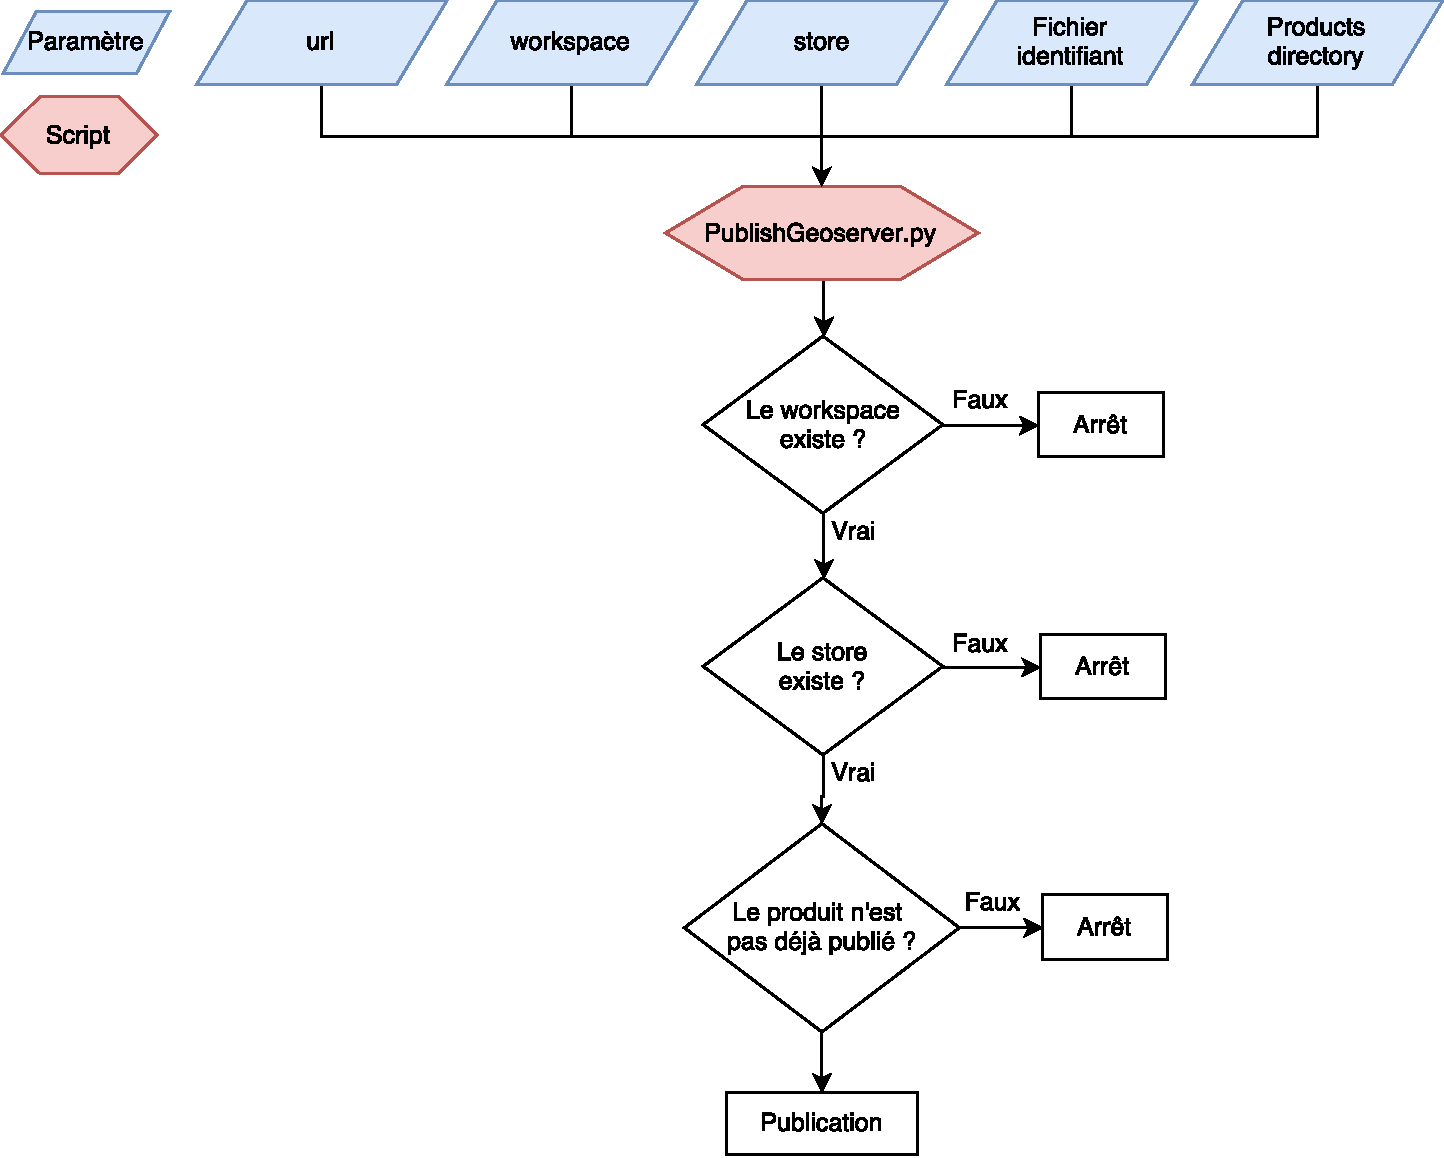
\includegraphics[scale=0.5]{img/orgPublication.pdf}
\caption{Organigramme des étapes pour la publication des indices sur un GeoServer.}
\label{orgPublication}
\end{figure}

Ainsi, la publication passe par plusieurs test afin de contrôler si le workspace, le store et la couche existent déjà (figure \ref{orgPublication}). Dans les deux premiers test, il n'est pas possible de publier la couche en leur absence et le troisième test évite de publier plusieurs fois la même image.\smallbreak
Si les tests sont réussis, alors cette commande est exécutée pour publier l'image :\newline 
\verb!"curl -v -u login:password -XPOST -H 'Content-type: text/plain'!\newline \verb!-d 'file://data/NDVI_YYYYMMDD.tif' 'http://geoserver/rest!\newline \verb!/workspaces/workspace/coveragestores/store/external.imagemosaic'"!

\section{Perspectives}

Les produits diffusés actuellement sur GéoBretagne possèdent plusieurs limites :
\begin{itemize}
\item la résolution spatiale de MODIS n'est pas adaptée au paysage Breton particulièrement fragmenté. Il n'est donc pas possible d'observer les bosquets, petites parcelles et les haies, entre autres. Il est donc envisagé d'utiliser le capteur Landsat avec une résolution spatiale de 30 mètres et une bande dans l'infrarouge thermique (critère obligatoire).
\item dans le cas du produit EF MODIS et grâce à la série temporelle, avec un pas de temps court, il serait intéressant de calculer les données manquantes sur le territoire afin d'avoir constamment de la données (probablement par interpolation entre plusieurs dates).
\item lors des prétraitements, il serait nécessaire de détecter et supprimer les nuages qui faussent les valeurs des produits.
\end{itemize}

Pour finir, il est nécessaire de gérer l'exécution automatique des scripts.

\section{Bibliographie}

\begin{itemize}
\item Bastiaanssen W.G.M., Ali, S. (2003). "A new crop yield forecasting model based on satellite measurements applied across the Indus Basin, Pakistan". Agric. Ecosyst. Environ. 94, pp.321–340.
\item Gao B.-C. (1996). "NDWI : A  Normalized  Difference  Water  Index  for  remote  sensing  of vegetation liquid water from space", Proceeding of SPIE.Vol.58, no.3, pp.257-266.
\item Morton, D. C., DeFries, R. S., Shimabukuro, Y. E., Anderson, L. O., Arai, E., del Bon Espirito-Santo, F.,  Freitas,  R.  et  Morisette,  J.,  (2006). "Cropland expansion changes deforestation dynamics in the southern Brazilian Amazon", Proceedings of the National Academy of Sciences, 103(39):14637. 
\item Nutini F., Boschetti M., Candiani G., Bocchi S., Brivio P.A., (2014). "Evaporative Fraction as an indicator of moisture condition and water stress status in semi-arid rangeland ecosystems". Remote sens., 6, pp.6300-6323.
\item Patakamuri S.K., Agrawal S., Krishnaveni M. (2014). "Time-series analysis of MODIS NDVI data along with ancillary data for land use/land cover mapping of Uttarakhand". The International Archives of the Photogrammetry, Remote Sensing and Spatial Information Sciences. XL-8, ISPRS Technical Commission VIII Symposium, pp.1491–1500
\item Roerink G., Su Z., Menenti M. (2000). "S-SEBI: A simple remote sensing algorithm to estimate the surface energy balance". Phys. Chem. Earth Part B 25, pp.147–157.
\item Rouse and Haas, (1973). "Monitoring vegetation systems in the great plain with ERTS", Third ERTS Symposium, Washington DC: NASA, no.1, pp.309-317.
\item Tucker, (1979). "Red and photographic infrared linear combinations for monitoring vegetation", Remote Sensing of the Environment, no.8, pp.127–150. 
\item Wardlow, B.D., Kastens, J.H. et Egbert, S.L. (2006). "Using USDA crop progress data for the evaluation of greenup onset date calculated from MODIS 250meter data", Photogrammetric Engineering and Remote Sensing 72(11), 1225-1234. 
\end{itemize}

\end{document}